\chapter*{Versuch 4: Widerstandsmessung mittels Vierdrahtmethode}

\subsection*{Ziel des Versuchs}

\section*{Versuchsdurchführung}

\subsection{Versuchsaufbau}

\begin{figure}[H]
	\centering
	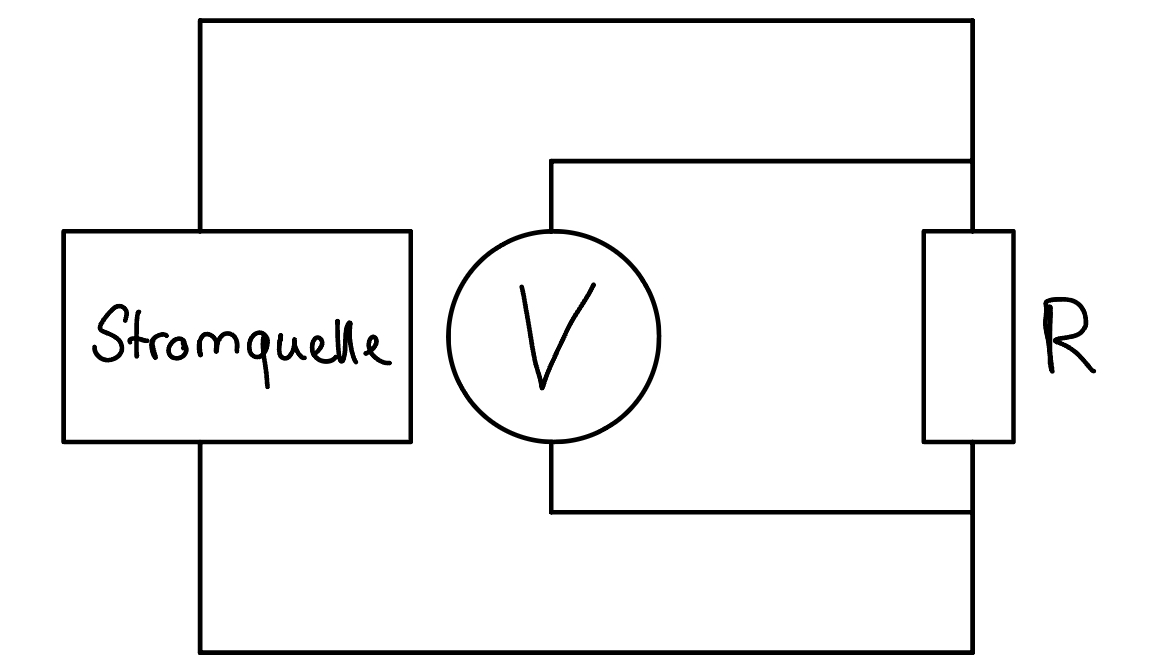
\includegraphics[height=7cm]{images/Versuch4/Schaltskizze.jpeg}
	\caption{Schaltungsskizze}
	\label{fig: Schaltungsskizze}
\end{figure}

XXXXXX Schaltungsaufbau XXXXXX

Durch diesen Aufbau kann man am Voltmeter, bzw. dem Digital-Multimeter,
den Widerstand R errechnen. Dieser berechnet sich nach folgender Formel:

\begin{equation}
    R = \frac{U}{I}
    \label{eq:R}
\end{equation}